\section{Results}

The claim-level ledger below maps the paper's four claims to their principal
evidence anchors. The full artifact index is in Appendix~\ref{app:artifacts}.
This section emphasizes each result's supported scope.

{\small
\paragraph{Claim-level evidence ledger.}
\begin{enumerate}
\item The frozen oracle sweep, noisy extractor-quality gate, and noisy
same-stream policy comparison all point to the same attribution story. All 108
frozen oracle deltas matched. The 7B gate blocked a false unlock. The
32B-gated comparison supports only the named mechanisms reported below.
\item The formal counterexample and internal canonical-id diagnostic show the
metric gap. Five of seven comparison rows pass the B-cubed floor while exact
canonical-id match is below 5 percent. The AMB LoCoMo replay uses third-party
outputs to show when the needed evidence was already in context and when rank
still mattered.
\item The LongMemEval v1 probe passes its methodology gates, but CQ minus
Reflection on \code{all_hit_at_50} is -1.0 in all three cells. The result is a
stable base-CQ evidence-completeness loss.
\item In the pending multi-evidence follow-up, plural pending readout moves
base CQ from 0/71 to 71/71 on the primary cell. Capped Reflection falls from
71/71 to 0/71. This pins the local failure on the answer read interface.
\end{enumerate}
}

\subsection{Oracle Results}

The frozen mechanism-diverse oracle sweep matched all preregistered deltas. CQ
and the ADD/UPDATE/NOOP eager-write baseline tied on aggregate answer correctness, false
assertion, poison promotion, clean durable displacement, and leakage. CQ's
narrower advantage was lower premature promotion, especially on
false-corroboration mixed-source rows. The result supports staged promotion as
a way to reduce premature durable commitment under oracle inputs. It does not
show broad answer-quality superiority over the ADD/UPDATE/NOOP eager-write
baseline.

The adversarial upstream-noise sweep is similarly mixed. CQ wins retraction,
witness conflict, scope narrowing, and pending competition, but loses temporal
skew. The post-hoc dated-evidence repair turns base CQ's temporal-skew
abstention into a correct answer from fresher dated evidence and preserves the
four original wins. The CQ-vs-Reflection win criterion remains unmet because
Reflection also lands at the correctness ceiling.

\subsection{Noisy Component Gate and Policy Comparison}

The component gate demonstrates why aggregate extractor metrics are
insufficient. The locked 7B row passed prompt-regression, determinism, aggregate
confidence-bound gates, and aggregate observed gates. It still stayed locked
because it had 45 primary scenario errors, eight per-family observed failures,
and three frozen-sentinel observed failures. An aggregate-only rule would have
authorized a false noisy policy comparison.

The preregistered 32B rows cleared the gate and licensed the noisy
same-stream policy comparison. The support is narrow:
CQ wins against \reflection{} on forced contradiction
(delta +0.93, lower confidence bound +0.88) and preference drift (delta +0.13,
lower confidence bound +0.07), records no countable directional losses, ties
the ADD/UPDATE/NOOP eager-write baseline on frozen sentinel primary metrics,
and has no replicate contradictions. The mechanism audit narrows this. Forced
contradiction survives cleanly, preference drift survives partially, and the
remaining rows stay null, descriptive, or bounded by component evidence.

\begin{figure}[t]
\centering
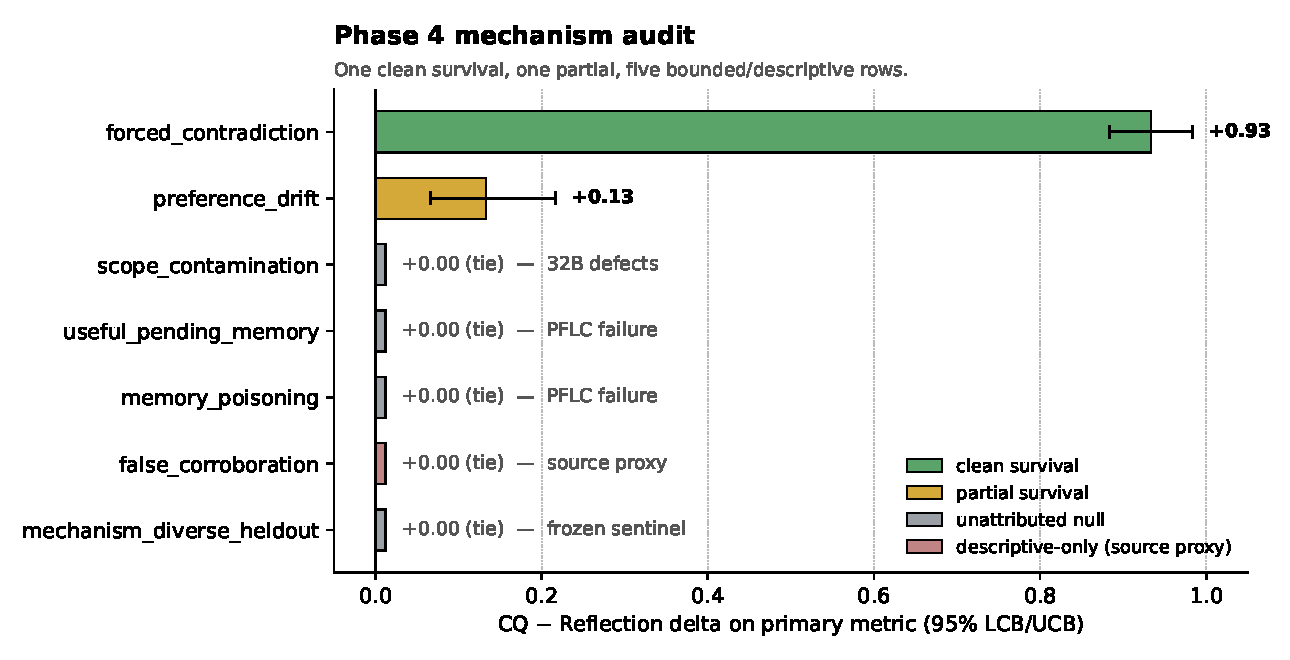
\includegraphics[width=0.92\linewidth]{figures/phase4_mechanism_audit}
\caption{Noisy same-stream policy comparison mechanism audit summary. Only forced contradiction survives
cleanly. Preference drift is partial, and other rows remain bounded,
diagnostic, or descriptive evidence (component defects, lookup-contract
failures, the descriptive-only event-source proxy for false corroboration, or
the frozen-sentinel held-out tie).}
\label{fig:phase4-audit}
\end{figure}

\subsection{Lookup Diagnostic and PFLC}

The lookup diagnostic adds a second diagnostic layer to several tied rows. On
\splitcode{useful\_\allowbreak pending\_\allowbreak memory},
\splitcode{memory\_\allowbreak poisoning},
\splitcode{false\_\allowbreak corroboration}, and the frozen sentinel, B-cubed
F1 is at or near 1.00 while exact
policy-query canonical-id agreement is 0.00. The locked alias-normalized
variant also stays at zero on those rows. The diagnostic does not replace the
mechanism-audit labels in Figure~\ref{fig:phase4-audit}: the
\splitcode{false\_\allowbreak corroboration} row still describes the extractor
surface rather than the policy direction. The mechanism-diverse row remains
the frozen sentinel aggregate, and the policy verdict does not change. It shows
that the extractor can look cluster-correct while the policy cannot name the
stored claim it must address.

The field-level PFLC work generalizes this observation. Identity-PFLC names the
memory-state gap: clustering, retrieval, and answer-accuracy metrics can expose
good groups, relevant content, or correct text while failing to certify the
governable evidence handle. The formal counterexamples live in
Appendix~\ref{app:pflc-gap}. The four-anchor survey over LongMemEval,
Mem0/LoCoMo, MemoryAgentBench, and MemBench splits on artifact accessibility:
most released baseline outputs are artifact-blocked, but a subset of published
Agent Memory Benchmark (AMB) LoCoMo runs expose recoverable per-question
evidence ids and support a published-output PFLC replay. The split is
summarized below. Benchmark-targeted synthetic counterexample rows ship
alongside.

\subsection{PFLC Decomposes Published LoCoMo Memory-Benchmark Outputs}
\label{sec:amb-replay}

Across the surveyed memory-benchmark artifacts, public outputs divide cleanly
into two classes. Most rows, including Mem0's \code{memory-benchmarks} platform,
A-MEM/AgenticMemory, SNAP LoCoMo RAG, Backboard, MemoryLake, Engram, and
external AMB comparison rows for Mem0, Zep, Letta, LangMem, and MemoryBank, do
not commit per-question retrieved context, retrieved memory ids, or LoCoMo
evidence ids in their released artifacts, and so admit no published-output
PFLC replay. Three AMB LoCoMo runs do: Hindsight (1{,}540 cases),
hybrid-search (1{,}540), and Cognee (152). Each injects per-question context
whose source blocks carry recoverable LoCoMo \code{dia_id}s, enabling a
context-derived PFLC replay against the official LoCoMo \code{qa[].evidence}
field.

\begin{table}[h]
\centering
\caption{Published-output PFLC on AMB LoCoMo runs (lookup-relevant denominator).}
\label{tab:amb-pflc}
\small
\begin{tabular}{lrrrrr}
\toprule
Run & Scored & Lookup-rel. & PFLC@10 & PFLC@20 & PFLC@50 \\
\midrule
AMB \code{locomo-hindsight}  & 1{,}540 & 1{,}536 & 65.8\% & 83.1\% & 97.6\% \\
AMB \code{hybrid-search}     & 1{,}540 & 1{,}536 & 64.8\% & 75.7\% & 90.5\% \\
AMB \code{cognee}            & 152     & 150     & 60.0\% & 73.3\% & 92.0\% \\
\bottomrule
\end{tabular}
\end{table}

The replayable runs do not collapse at the lookup step. They decompose
LoCoMo's aggregate answer accuracy into three components that the aggregate
conflates. For example, AMB hybrid-search produces 276 cases where the answer
is wrong while every gold evidence \code{dia_id} is already present in the
emitted context by PFLC@50, isolating an answering or judging residual from
a retrieval-contract residual. Conversely, 100 cases are correct while all
gold evidence is missing at PFLC@50, flagging answer success not fully backed
by the LoCoMo evidence contract as scored here. PFLC@10 and PFLC@20 carry the
rank-sensitivity signal because Hindsight averages 36{,}235 context tokens
per question.

The operational claim is therefore narrow: once per-question context is
published, PFLC can tell whether the answer had the needed evidence in context,
whether rank or context limits mattered, or whether the remaining error sits
downstream in answering or judging. This replay does not certify that a memory
policy can name its own governable evidence handle. The internal canonical-id
diagnostic tests that separate question. Without per-question artifacts, the
same decomposition is impossible, which is why the artifact-blocked subset
remains the headline survey gap.

\subsection{Controlled Readout-Cardinality Probe on LongMemEval v1}

The LongMemEval v1 probe produces an inspectable negative external result. The
run covers 1,935 policy/cell/case rows across
\code{primary_contract}, \code{path_a_only_denominator}, and
\code{path_b_only_denominator}. Candidate-stream hash invariants pass in all
cells. The headline result is shown in Table~\ref{tab:x4}.

\begin{table}[h]
\centering
\caption{LongMemEval v1 result: CQ-vs-Reflection on evidence completeness.}
\label{tab:x4}
\begin{tabular}{lrr}
\toprule
Cell & \code{all_hit_at_50} delta & \code{any_hit_at_50} delta\\
\midrule
\code{primary_contract} & -1.0 & 0.0\\
\code{path_a_only_denominator} & -1.0 & 0.0\\
\code{path_b_only_denominator} & -1.0 & 0.0\\
\bottomrule
\end{tabular}
\end{table}

The stable sign fires the preregistered-gate condition, but the sign is
negative. CQ retrieves at least one gold evidence session in every case and
therefore ties eager baselines on \code{any_hit_at_50}, which asks whether at
least one required gold session is returned. It never retrieves both evidence
sessions, so it loses \code{all_hit_at_50}. The methodology gate passes, but the
probe is CQ-negative and isolates a pending-readout gap.

\begin{figure}[H]
\centering
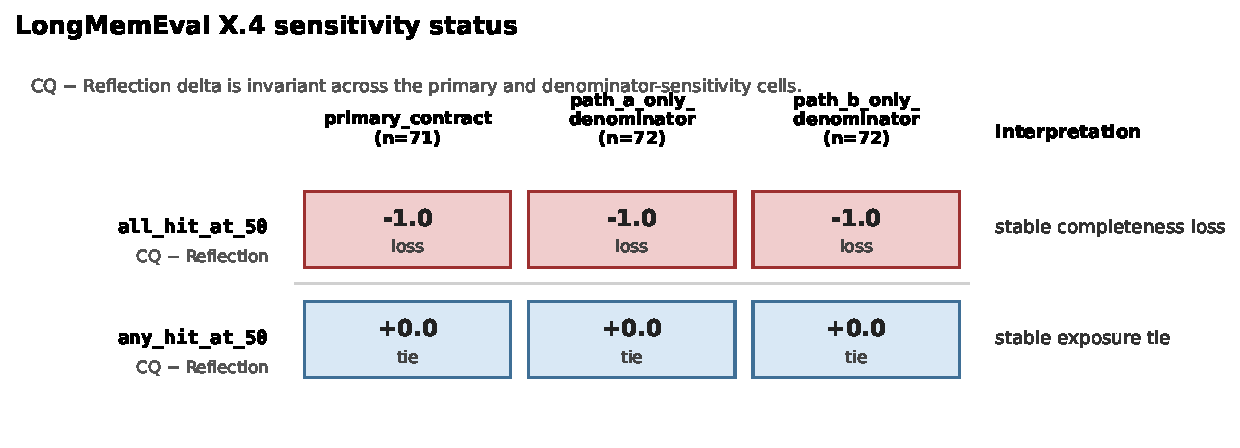
\includegraphics[width=0.90\linewidth]{figures/longmemeval_x4_cells}
\caption{LongMemEval v1 sensitivity status. The CQ-vs-Reflection delta is
stable across the primary and denominator-sensitivity cells: -1.0 on
\code{all_hit_at_50} and 0.0 on \code{any_hit_at_50}.}
\label{fig:x4-cells}
\end{figure}

\subsection{All-Hit Metric Floor}

The LongMemEval v1 probe is evidence-only: in the committed
rows, the observed unique session-id pool for each scored case contains exactly
the two gold evidence sessions. A scorer-only random floor therefore exposes a
sharp cardinality property of the metric. A singleton readout has zero chance
to satisfy \code{all_hit_at_50}. A random two-session readout has a 100\%
closed-form floor in all three cells, confirmed by five seeded draws per case.
This does not weaken the original base-CQ loss, because base CQ returns only
one session. It does bound the follow-up interpretation. The plural-pending
readout variant succeeds on v1 by exposing plural same-slot evidence rather
than by demonstrating broad distractor-heavy retrieval quality.

% Generated by scripts/compute_all_hit_at_50_random_floor.py.
\begin{table}[h]
\centering
\caption{Scorer-only random-readout floor for LongMemEval \code{all_hit_at_50}.}
\label{tab:all-hit-random-floor}
\small
\resizebox{\linewidth}{!}{%
\begin{tabular}{lrrrrrr}
\toprule
Cell & Cases & Mean pool & Mean gold & Random $r{=}1$ & Random $r{=}2$ & 5-seed $r{=}2$ band \\
\midrule
path\_a\_only\_denominator & 72 & 2.00 & 2.00 & 0.0\% & 100.0\% & 100.0\%--100.0\% \\
path\_b\_only\_denominator & 72 & 2.00 & 2.00 & 0.0\% & 100.0\% & 100.0\%--100.0\% \\
primary\_contract & 71 & 2.00 & 2.00 & 0.0\% & 100.0\% & 100.0\%--100.0\% \\
\bottomrule
\end{tabular}
}
\end{table}


\subsection{Pending Multi-Evidence Follow-Up}

The follow-up is structured around two paired predictions. CQ should close the
\code{all_hit_at_50} gap if it is allowed to return all eligible same-slot
pending candidates. Reflection should reproduce the original base-CQ loss if it
keeps its winning write path but is capped to one durable candidate id at answer
time. The storage, adapter, judge, and headline metric stay fixed. The
Reflection control is the load-bearing half because it reproduces the loss on a
baseline that previously won the metric.

Both predictions hold (Table~\ref{tab:y}). Plural pending readout moves base
CQ from $0/71$ to $71/71$ in the primary cell. Capping Reflection moves it
from $71/71$ to $0/71$ in the same cell. The pattern is stable across both
denominator-sensitivity cells.

\begin{table}[h]
\centering
\caption{Pending multi-evidence follow-up on \code{all_hit_at_50}: the
repair and the symmetric falsifier.}
\label{tab:y}
\begin{tabular}{lrrrr}
\toprule
Cell & Base CQ & Follow-up CQ & Reflection & Capped Reflection\\
\midrule
\code{primary_contract} & 0/71 & 71/71 & 71/71 & 0/71\\
\code{path_a_only_denominator} & 0/72 & 72/72 & 72/72 & 0/72\\
\code{path_b_only_denominator} & 0/72 & 72/72 & 72/72 & 0/72\\
\bottomrule
\end{tabular}
\end{table}

The internal regression gate reports maximum checked overall delta 0.0 across
forced contradiction, preference drift, mechanism-diverse held-out,
adversarial upstream noise, and evidence-conflict spectrum. The committed
metrics are aggregate policy rows rather than per-scenario CQ-Multi-vs-base-CQ
pairs, so the regression table reports per-family overall deltas only.

% Generated by scripts/build_cqmulti_per_row_regression_table.py.
\begin{table}[h]
\centering
\caption{CQ-Multi internal regression replay over aggregate policy rows.}
\label{tab:cqmulti-regression}
\small
\begin{tabular}{lrrrr}
\toprule
Family & Scenarios & Checked metrics & Max $|\Delta|$ & Non-zero deltas \\
\midrule
Forced contradiction & 25 & 26 & 0.000000 & none \\
Preference drift & 25 & 26 & 0.000000 & none \\
Mechanism-diverse held-out & 3 & 26 & 0.000000 & none \\
Adversarial upstream noise & 25 & 26 & 0.000000 & none \\
Evidence-conflict spectrum & 25 & 26 & 0.000000 & none \\
\bottomrule
\end{tabular}
\vspace{2pt}
\begin{minipage}{0.92\linewidth}
\footnotesize
The aggregate maximum checked overall delta is 0.000000. The committed CQ-Multi
CSV artifacts contain policy-summary rows, so this table reports per-family
overall deltas only; no per-scenario confidence intervals are inferred from
these aggregate files.
\end{minipage}
\end{table}


Focused
negative-control tests confirm that below-floor poisoned siblings, contested
siblings, wrong-scope siblings, mirrored-source weak siblings, and demoted
siblings are not returned by plural pending lookup. With the symmetric
falsifier holding, the follow-up supports the read-interface explanation. It
does not support a richer CQ-only memory substrate or broader CQ-vs-Reflection
superiority.

% Cardinality-repair follow-up (repo: Phase Y; replaces phase_y_cardinality_control.png).
%
% Usage: see externalization_protocol.tex for the required preamble.
% Replace the existing 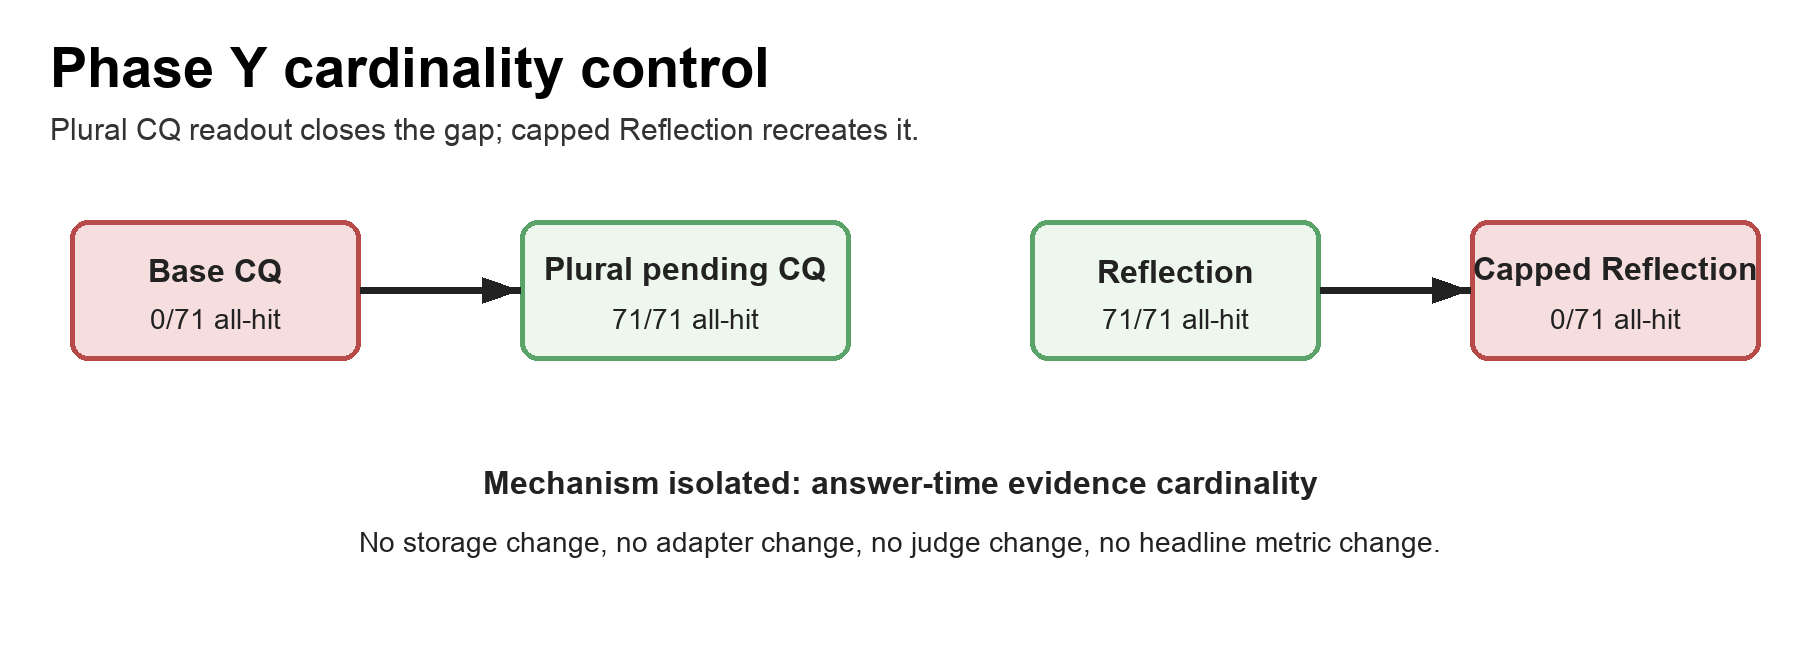
\includegraphics{figures/phase_y_cardinality_control.png}
% in paper/sections/results.tex with
%   % Cardinality-repair follow-up (repo: Phase Y; replaces phase_y_cardinality_control.png).
%
% Usage: see externalization_protocol.tex for the required preamble.
% Replace the existing 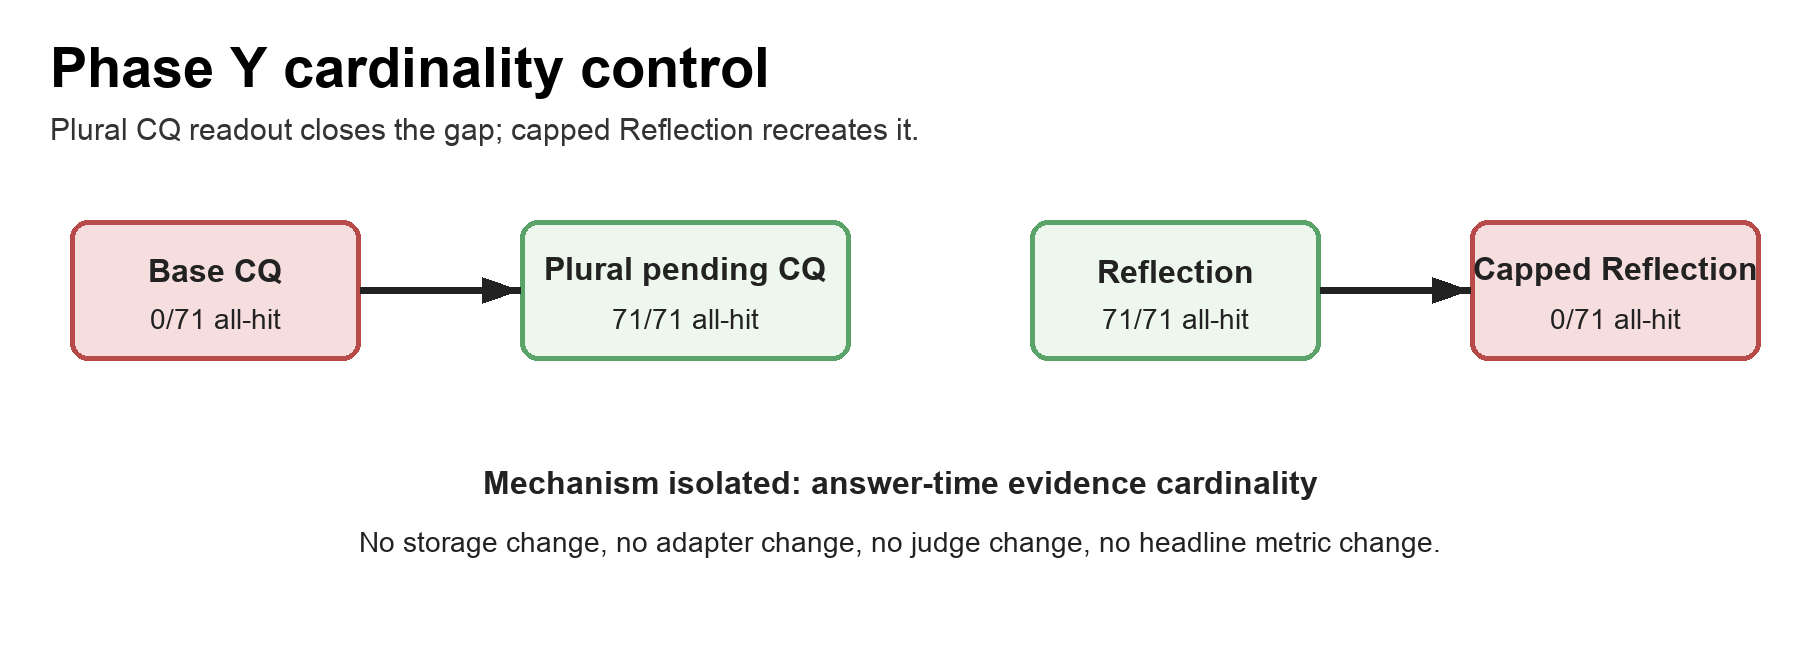
\includegraphics{figures/phase_y_cardinality_control.png}
% in paper/sections/results.tex with
%   % Cardinality-repair follow-up (repo: Phase Y; replaces phase_y_cardinality_control.png).
%
% Usage: see externalization_protocol.tex for the required preamble.
% Replace the existing 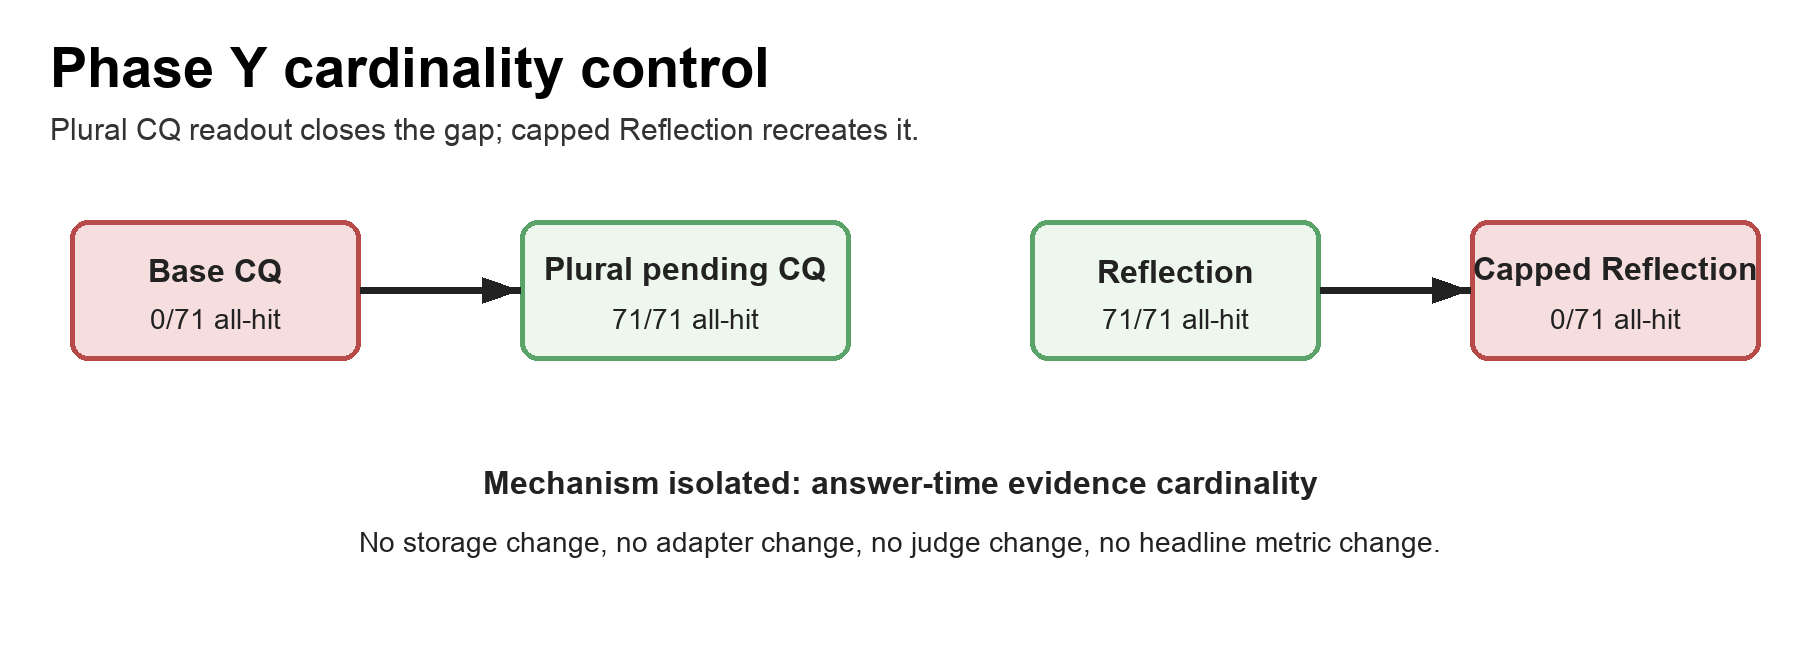
\includegraphics{figures/phase_y_cardinality_control.png}
% in paper/sections/results.tex with
%   \input{figures/phase_y_cardinality_control.tex}
%
% Sources for the depicted numbers:
%   docs/cq_pending_multi_evidence_results.md (primary_contract cell)
%   data/external/longmemeval/transfer_followup_per_case_rows.csv
%   cq/memory/cq_pending_multi_evidence.py
%   cq/memory/reflection_eager_write_cardinality_capped.py

\begin{figure}[t]
\centering
\resizebox{\linewidth}{!}{%
\begin{tikzpicture}[
  font=\small,
  node distance=6mm,
  state/.style={
    rounded corners=3pt, draw, line width=0.7pt,
    minimum width=32mm, minimum height=14mm,
    align=center, inner sep=2mm,
  },
  lose/.style={state, draw=red!60!black,   fill=red!7},
  win/.style ={state, draw=green!55!black, fill=green!8},
  swap/.style={
    -{Stealth[length=2.4mm]}, line width=0.8pt,
  },
  swaplabel/.style={
    font=\scriptsize, align=center,
    fill=white, inner sep=1pt,
  },
  caption/.style={font=\small\bfseries, align=center},
  subcap/.style={font=\footnotesize, align=center, color=black!65},
  panel/.style={
    rounded corners=4pt, draw=black!25, line width=0.4pt,
    inner sep=4mm,
  },
]

% ===== Left half: CQ swap (lose -> win) =====
\node[lose] (cq0) {\textbf{Base CQ}\\$0\,/\,71$ all\_hit\_at\_50};
\node[win, right=26mm of cq0] (cq1) {\textbf{Plural pending CQ}\\$71\,/\,71$ all\_hit\_at\_50};

\draw[swap] (cq0.east) -- node[swaplabel, above]
  {pending readout:\\[-1pt]\textbf{1} $\to$ \textbf{all eligible}}
  (cq1.west);

\node[subcap, below=2pt of cq0] {(loses completeness)};
\node[subcap, below=2pt of cq1] {(closes completeness)};

% ===== Right half: Reflection swap (win -> lose) =====
\node[win, right=44mm of cq1] (rf0) {\textbf{Reflection}\\$71\,/\,71$ all\_hit\_at\_50};
\node[lose, right=26mm of rf0] (rf1) {\textbf{Capped Reflection}\\$0\,/\,71$ all\_hit\_at\_50};

\draw[swap] (rf0.east) -- node[swaplabel, above]
  {answer readout:\\[-1pt]\textbf{all} $\to$ \textbf{1}}
  (rf1.west);

\node[subcap, below=2pt of rf0] {(wins completeness)};
\node[subcap, below=2pt of rf1] {(reproduces loss)};

% ===== Vertical separator between the two swaps =====
\draw[draw=black!20, dashed, line width=0.4pt]
  ($(cq1.east)!0.5!(rf0.west)+(0,18mm)$) -- ($(cq1.east)!0.5!(rf0.west)+(0,-32mm)$);

% ===== Section captions above each swap =====
\node[caption, above=10mm of cq0.north east, anchor=center,
      xshift=22mm] (cqcap)
  {CQ: expose plural pending evidence};
\node[caption, above=10mm of rf0.north east, anchor=center,
      xshift=22mm] (rfcap)
  {Reflection: cap durable readout to one id};

% ===== Bottom takeaway =====
\node[caption, below=18mm of cq1.south east, anchor=north, xshift=22mm]
  (takeaway) {Mechanism isolated: answer-time evidence cardinality.};
\node[subcap, below=1mm of takeaway]
  {No storage change. No adapter change. No judge change. No headline-metric change.};

\end{tikzpicture}%
}
\caption{Cardinality-repair follow-up. Changing the CQ pending-readout
  cardinality from singleton to plural converts a $0/71$ loss into a $71/71$
  win on \texttt{all\_hit\_at\_50} in the primary cell. Capping the durable
  Reflection readout to a single id reproduces the original CQ loss with the
  same magnitude. The symmetric swap isolates answer-time evidence
  cardinality as the responsible interface variable; nothing else in the
  pipeline changes.}
\label{fig:phase-y-cardinality}
\end{figure}

%
% Sources for the depicted numbers:
%   docs/cq_pending_multi_evidence_results.md (primary_contract cell)
%   data/external/longmemeval/transfer_followup_per_case_rows.csv
%   cq/memory/cq_pending_multi_evidence.py
%   cq/memory/reflection_eager_write_cardinality_capped.py

\begin{figure}[t]
\centering
\resizebox{\linewidth}{!}{%
\begin{tikzpicture}[
  font=\small,
  node distance=6mm,
  state/.style={
    rounded corners=3pt, draw, line width=0.7pt,
    minimum width=32mm, minimum height=14mm,
    align=center, inner sep=2mm,
  },
  lose/.style={state, draw=red!60!black,   fill=red!7},
  win/.style ={state, draw=green!55!black, fill=green!8},
  swap/.style={
    -{Stealth[length=2.4mm]}, line width=0.8pt,
  },
  swaplabel/.style={
    font=\scriptsize, align=center,
    fill=white, inner sep=1pt,
  },
  caption/.style={font=\small\bfseries, align=center},
  subcap/.style={font=\footnotesize, align=center, color=black!65},
  panel/.style={
    rounded corners=4pt, draw=black!25, line width=0.4pt,
    inner sep=4mm,
  },
]

% ===== Left half: CQ swap (lose -> win) =====
\node[lose] (cq0) {\textbf{Base CQ}\\$0\,/\,71$ all\_hit\_at\_50};
\node[win, right=26mm of cq0] (cq1) {\textbf{Plural pending CQ}\\$71\,/\,71$ all\_hit\_at\_50};

\draw[swap] (cq0.east) -- node[swaplabel, above]
  {pending readout:\\[-1pt]\textbf{1} $\to$ \textbf{all eligible}}
  (cq1.west);

\node[subcap, below=2pt of cq0] {(loses completeness)};
\node[subcap, below=2pt of cq1] {(closes completeness)};

% ===== Right half: Reflection swap (win -> lose) =====
\node[win, right=44mm of cq1] (rf0) {\textbf{Reflection}\\$71\,/\,71$ all\_hit\_at\_50};
\node[lose, right=26mm of rf0] (rf1) {\textbf{Capped Reflection}\\$0\,/\,71$ all\_hit\_at\_50};

\draw[swap] (rf0.east) -- node[swaplabel, above]
  {answer readout:\\[-1pt]\textbf{all} $\to$ \textbf{1}}
  (rf1.west);

\node[subcap, below=2pt of rf0] {(wins completeness)};
\node[subcap, below=2pt of rf1] {(reproduces loss)};

% ===== Vertical separator between the two swaps =====
\draw[draw=black!20, dashed, line width=0.4pt]
  ($(cq1.east)!0.5!(rf0.west)+(0,18mm)$) -- ($(cq1.east)!0.5!(rf0.west)+(0,-32mm)$);

% ===== Section captions above each swap =====
\node[caption, above=10mm of cq0.north east, anchor=center,
      xshift=22mm] (cqcap)
  {CQ: expose plural pending evidence};
\node[caption, above=10mm of rf0.north east, anchor=center,
      xshift=22mm] (rfcap)
  {Reflection: cap durable readout to one id};

% ===== Bottom takeaway =====
\node[caption, below=18mm of cq1.south east, anchor=north, xshift=22mm]
  (takeaway) {Mechanism isolated: answer-time evidence cardinality.};
\node[subcap, below=1mm of takeaway]
  {No storage change. No adapter change. No judge change. No headline-metric change.};

\end{tikzpicture}%
}
\caption{Cardinality-repair follow-up. Changing the CQ pending-readout
  cardinality from singleton to plural converts a $0/71$ loss into a $71/71$
  win on \texttt{all\_hit\_at\_50} in the primary cell. Capping the durable
  Reflection readout to a single id reproduces the original CQ loss with the
  same magnitude. The symmetric swap isolates answer-time evidence
  cardinality as the responsible interface variable; nothing else in the
  pipeline changes.}
\label{fig:phase-y-cardinality}
\end{figure}

%
% Sources for the depicted numbers:
%   docs/cq_pending_multi_evidence_results.md (primary_contract cell)
%   data/external/longmemeval/transfer_followup_per_case_rows.csv
%   cq/memory/cq_pending_multi_evidence.py
%   cq/memory/reflection_eager_write_cardinality_capped.py

\begin{figure}[t]
\centering
\resizebox{\linewidth}{!}{%
\begin{tikzpicture}[
  font=\small,
  node distance=6mm,
  state/.style={
    rounded corners=3pt, draw, line width=0.7pt,
    minimum width=32mm, minimum height=14mm,
    align=center, inner sep=2mm,
  },
  lose/.style={state, draw=red!60!black,   fill=red!7},
  win/.style ={state, draw=green!55!black, fill=green!8},
  swap/.style={
    -{Stealth[length=2.4mm]}, line width=0.8pt,
  },
  swaplabel/.style={
    font=\scriptsize, align=center,
    fill=white, inner sep=1pt,
  },
  caption/.style={font=\small\bfseries, align=center},
  subcap/.style={font=\footnotesize, align=center, color=black!65},
  panel/.style={
    rounded corners=4pt, draw=black!25, line width=0.4pt,
    inner sep=4mm,
  },
]

% ===== Left half: CQ swap (lose -> win) =====
\node[lose] (cq0) {\textbf{Base CQ}\\$0\,/\,71$ all\_hit\_at\_50};
\node[win, right=26mm of cq0] (cq1) {\textbf{Plural pending CQ}\\$71\,/\,71$ all\_hit\_at\_50};

\draw[swap] (cq0.east) -- node[swaplabel, above]
  {pending readout:\\[-1pt]\textbf{1} $\to$ \textbf{all eligible}}
  (cq1.west);

\node[subcap, below=2pt of cq0] {(loses completeness)};
\node[subcap, below=2pt of cq1] {(closes completeness)};

% ===== Right half: Reflection swap (win -> lose) =====
\node[win, right=44mm of cq1] (rf0) {\textbf{Reflection}\\$71\,/\,71$ all\_hit\_at\_50};
\node[lose, right=26mm of rf0] (rf1) {\textbf{Capped Reflection}\\$0\,/\,71$ all\_hit\_at\_50};

\draw[swap] (rf0.east) -- node[swaplabel, above]
  {answer readout:\\[-1pt]\textbf{all} $\to$ \textbf{1}}
  (rf1.west);

\node[subcap, below=2pt of rf0] {(wins completeness)};
\node[subcap, below=2pt of rf1] {(reproduces loss)};

% ===== Vertical separator between the two swaps =====
\draw[draw=black!20, dashed, line width=0.4pt]
  ($(cq1.east)!0.5!(rf0.west)+(0,18mm)$) -- ($(cq1.east)!0.5!(rf0.west)+(0,-32mm)$);

% ===== Section captions above each swap =====
\node[caption, above=10mm of cq0.north east, anchor=center,
      xshift=22mm] (cqcap)
  {CQ: expose plural pending evidence};
\node[caption, above=10mm of rf0.north east, anchor=center,
      xshift=22mm] (rfcap)
  {Reflection: cap durable readout to one id};

% ===== Bottom takeaway =====
\node[caption, below=18mm of cq1.south east, anchor=north, xshift=22mm]
  (takeaway) {Mechanism isolated: answer-time evidence cardinality.};
\node[subcap, below=1mm of takeaway]
  {No storage change. No adapter change. No judge change. No headline-metric change.};

\end{tikzpicture}%
}
\caption{Cardinality-repair follow-up. Changing the CQ pending-readout
  cardinality from singleton to plural converts a $0/71$ loss into a $71/71$
  win on \texttt{all\_hit\_at\_50} in the primary cell. Capping the durable
  Reflection readout to a single id reproduces the original CQ loss with the
  same magnitude. The symmetric swap isolates answer-time evidence
  cardinality as the responsible interface variable; nothing else in the
  pipeline changes.}
\label{fig:phase-y-cardinality}
\end{figure}

